\documentclass[11pt, a4paper]{article}

\usepackage[top = 1 in, bottom = 1 in, left = 1 in, right = 1 in]{geometry}

\usepackage{amsmath, amssymb, amsfonts}

\usepackage{amsthm}
\theoremstyle{definition}
\newtheorem{example}{Example}[subsection]

\usepackage{enumerate}
\usepackage{multirow}
\usepackage{hhline}
\usepackage{array}
\usepackage{longtable}
\usepackage{graphicx}
\usepackage{tabularray}
\usepackage{undertilde}
\usepackage{dingbat}
\usepackage{fontawesome5}
\usepackage[colorlinks=true, linkcolor=blue, urlcolor=blue]{hyperref}
\usepackage{tasks}
\usepackage{bbding}
\usepackage{twemojis}
% how to use bull's eye ----- \scalebox{2.0}{\twemoji{bullseye}}
\usepackage{customdice}
% how to put dice face ------ \dice{2}
\usepackage{bclogo}
\usepackage{simpsons}
\usepackage{tablefootnote}
\usepackage{figchild}
\usepackage{tikz}
\usepackage{pgfplots}
\pgfplotsset{compat=1.17}
\usetikzlibrary{arrows.meta}
\usepackage{xcolor}
\definecolor{darkgreen}{RGB}{0,100,0}

\title{MSMS 304 - Biostatistics \\[0.5em] Randomization}
\author{Ananda Biswas}
\date{Last updated : \today}


\begin{document}

\maketitle

\tableofcontents

\newpage

\section{Introduction}

Randomization is a process by which each participant has the same chance of being assigned to either intervention or control. Of course, neither trial participant nor investigator should know what the assignment will be before the participant's decision to enter the study. Otherwise, the benefits of randomization can be lost.

\begin{center}
\textit{Randomization tends to produce study groups comparable with respect to known as well as unknown risk factors, removes investigator bias in the allocation of participants, and guarantees that statistical tests will have valid false positive error rates.}
\end{center}

\section{Fixed Allocation Randomization}

Fixed allocation procedures assign the interventions to participants with a pre-specified probability, usually equal, and that allocation probability is not altered as the study progresses. Allocation to intervention and control groups should be equal unless there are compelling reasons to do otherwise. A number of methods exists by which fixed allocation is achieved and we review a few of them here.

\subsection{Simple Randomization}

One simple method is to toss an unbiased coin each time a participant is eligible to be randomized. For example, if the coin turns up heads, the participant is assigned to group A; if tails, to group B. Using this procedure, approximately one half of the participants will be 
in group A and one half in group B. \\[0.25em]

Table of random numbers, random number generation by computers are also common techniques for producing a randomization schedule. These most elementary methods of randomization are referred to as \textit{simple} or \textit{complete randomization}. \\[0.25em]

The \textit{advantage} of this simple randomization procedure is that it is easy to implement. The major \textit{disadvantage} is that, although in the long run the number of participants in each group will be in the proportion anticipated, at any point in the randomization, including the end, there could be a substantial imbalance. This is true particularly if the sample size is small. While such imbalances do not cause the statistical tests to be invalid, they do reduce ability to detect true differences between the two groups. In addition, such imbalances appear awkward and may lead to some loss of credibility for the trial, especially for the person not oriented to statistics.

\subsection{Block Randomization}

Blocked randomization, sometimes called permuted block randomization, is used in order to avoid serious imbalance in the number of participants assigned to each group – an imbalance that could occur in the simple randomization procedure. Blocked randomization guarantees that at no 
time during randomization will the imbalance be large and that at certain points the number of participants in each group will be equal. If participants are randomly assigned with equal probability to groups $A$ or $B$, then for each block of even size \textit{e.g.} $(4, 6, or \, 8)$, one half of the participants will be assigned to $A$ and the other half to $B$. The order in which the interventions are assigned in each block is randomized, and this process is repeated for consecutive 
blocks of participants until all participants are randomized. \\[0.25em]

\fcThermometerA[scale = 0.4, draw = blue, line width = 1.5] \textbf{An example :} Consider the case where a clinical trial was conducted to test the efficacy of Propranolol versus Nifedipine for reducing chest pain in patients with chronic stable angina. The investigators may want to ensure that after every fourth randomized participant, the number of participants in each intervention group is equal. Then, a block of size $4$ would be used, and the process would randomize the order in which two `Propranolol's and two `Nifedipine's are assigned for every consecutive group of four participants entering the trial. One may write down all the ways of arranging the groups and then randomize the 
order in which these combinations are selected. In the case of block size $4$, there are $^4C_2 = 6$ possible combinations of group assignments as listed below.

\begin{figure}[!htbp]
\centering
\includegraphics[scale=0.35]{block_randomization_blocks}
\end{figure}

One of these arrangements is selected at random and the four 
participants are assigned accordingly. This process is repeated as many times as needed. \\[0.5em]

Suppose we have $24$ patients to allocate, then the process will be as follows.

\begin{enumerate}[\text{Draw} 1.]
\item \textit{Select a block at random :} \textbf{Block 2} \\[0.1em]
\textit{Allocation Scheme :} Participant $1 \rightarrow $ Nifedipine, Participant $2 \rightarrow $ Propranolol,\\ Participant $3 \rightarrow $ Nifedipine, Participant $4 \rightarrow $ Propranolol.

\begin{figure}[!htbp]
\centering
\includegraphics[scale=0.35]{block_randomization_allocation_1}
\end{figure}

\newpage

\item \textit{Select a block at random :} \textbf{Block 4} \\[0.1em]
\textit{Allocation Scheme :} Participant $5 \rightarrow $ Nifedipine, Participant $6 \rightarrow $ Nifedipine,\\ Participant $7 \rightarrow $ Propranolol, Participant $8 \rightarrow $ Propranolol.

\begin{figure}[!htbp]
\centering
\includegraphics[scale=0.35]{block_randomization_allocation_2}
\end{figure}

\item \textit{Select a block at random :} \textbf{Block 6} \\[0.1em]
\textit{Allocation Scheme :} Participant $9 \rightarrow $ Nifedipine, Participant $10 \rightarrow $ Propranolol,\\ Participant $11 \rightarrow $ Propranolol, Participant $12 \rightarrow $ Nifedipine.

\begin{figure}[!htbp]
\centering
\includegraphics[scale=0.35]{block_randomization_allocation_3}
\end{figure}

\item \textit{Select a block at random :} \textbf{Block 1} \\[0.1em]
\textit{Allocation Scheme :} Participant $13 \rightarrow $ Propranolol, Participant $14 \rightarrow $ Nifedipine,\\ Participant $15 \rightarrow $ Propranolol, Participant $16 \rightarrow $ Nifedipine.

\begin{figure}[!htbp]
\centering
\includegraphics[scale=0.35]{block_randomization_allocation_4}
\end{figure}

\newpage

\item \textit{Select a block at random :} \textbf{Block 4} \\[0.1em]
\textit{Allocation Scheme :} Participant $17 \rightarrow $ Nifedipine, Participant $18 \rightarrow $ Nifedipine,\\ Participant $19 \rightarrow $ Propranolol, Participant $20 \rightarrow $ Propranolol.

\begin{figure}[!htbp]
\centering
\includegraphics[scale=0.35]{block_randomization_allocation_5}
\end{figure}

\item \textit{Select a block at random :} \textbf{Block 2} \\[0.1em]
\textit{Allocation Scheme :} Participant $21 \rightarrow $ Nifedipine, Participant $22 \rightarrow $ Propranolol,\\ Participant $23 \rightarrow $ Nifedipine, Participant $24 \rightarrow $ Propranolol.

\begin{figure}[!htbp]
\centering
\includegraphics[scale=0.35]{block_randomization_allocation_6}
\end{figure}

\end{enumerate}

Thus all $24$ participants are allocated. \\[0.1em]

Websites like \href{https://www.sealedenvelope.com/}{sealedenvelope.com} facilitate such randomization procedures. A demonstration with the same example we just discussed can be found \href{https://youtu.be/h7EyOibsLk0}{here}.

\newpage

\subsection{Stratified Randomization}

One of the objectives in allocating participants is to achieve \textit{between group comparability} of certain characteristics known as \textit{prognostic} or \textit{risk factors}. Measured at baseline, these are factors that correlate with subsequent participant response or outcome. Investigators may become concerned when prognostic factors are not evenly distributed between intervention and control groups. For any single study, especially a small study, there is no guarantee that all baseline characteristics will be similar in the two groups. Stratified randomization is a method that helps achieve comparability between the study groups for those factors considered.

Stratified randomization requires that the prognostic factors be measured either before or at the time of randomization. If a single factor is used, it is divided into two or more subgroups or strata (\textit{e.g.}, age $30-34$ years, $35-39$ years, $40-44$ years). 
If several factors are used, a stratum is formed by selecting one subgroup from each of them. The total number of strata is the product of the number of subgroups in each factor. The stratified randomization process involves measuring the level of the selected factors for a participant, determining to which stratum she belongs and 
performing the randomization within that stratum.

Within each stratum, the randomization process itself could be simple randomization, but in practice most clinical trials use some blocked randomization strategy. Under a simple randomization process, imbalances in the number in each group within the stratum could easily happen and thus defeat the purpose of the stratification.

As an example of stratified randomization with a block size of $4$, suppose an investigator wants to stratify on age, sex, and smoking history. One possible classification of the factors would be three 10-year age levels and three smoking levels.

\begin{table}[!htbp]
\def\arraystretch{1.5}
\begin{center}
\begin{tabular}{>{\centering}m{2.5cm}>{\centering}m{2.5cm}>{\centering\arraybackslash}m{3.5cm}}
\hline
Age(years) & Sex & Smoking history \\
\hline
\hline
\begin{enumerate}[1.]
\item $40-49$ \item $50-59$ \item $60-69$
\end{enumerate}
&
\begin{enumerate}[1.]
\item Male \item Female
\end{enumerate}
&
\begin{enumerate}[1.]
\item Current smoker \item Ex-smoker \item Never smoked
\end{enumerate} \\
\hline
\end{tabular}
\end{center}
\end{table}

Thus, the design has $3 \times 2 \times 3 = 18$ strata. \\[0.5em]


\fcThermometerB[scale = 0.4, draw = blue, line width = 1.5] \textbf{An demonstration :} Let us continue with our previous example of a clinical trial that was conducted to test the efficacy of Propranolol versus Nifedipine for reducing chest pain in patients with chronic stable angina. We remain consistent with blocks of size $4$. Here we take into account a single risk factor \textit{age} and consider two levels ``$<40$" and ``$>40$". Thus we segregate the participants into 2 strata. Suppose there are $24$ total participants among which $12$ have age $<40$ and rest $12$ have age $>40$. Let $SiPj$ denote the $j-$th participant in stratum $i$. \\[0.5em]


The randomization process is as follows : 

\newpage

\scalebox{2.0}{\twemoji{keycap: 1}} \hspace{0.1cm} First we allocate participants of stratum $1$.

\begin{enumerate}[\text{Draw} 1.]
\item \textit{Select a block at random :} \textbf{Block 4} \\[0.1em]
\textit{Allocation Scheme :} Participant $S1P1 \rightarrow $ Nifedipine, Participant $S2P2 \rightarrow $ Nifedipine,\\ Participant $S1P3 \rightarrow $ Propranolol, Participant $S1P4 \rightarrow $ Propranolol.

\begin{figure}[!htbp]
\centering
\includegraphics[scale=0.35]{stratified_block_randomization_stratum_1_allocation_1}
\end{figure}


\item \textit{Select a block at random :} \textbf{Block 1} \\[0.1em]
\textit{Allocation Scheme :} Participant $S1P5 \rightarrow $ Propranolol, Participant $S2P6 \rightarrow $ Nifedipine,\\ Participant $S1P7 \rightarrow $ Propranolol, Participant $S1P8 \rightarrow $ Nifedipine.

\begin{figure}[!htbp]
\centering
\includegraphics[scale=0.35]{stratified_block_randomization_stratum_1_allocation_2}
\end{figure}


\item \textit{Select a block at random :} \textbf{Block 3} \\[0.1em]
\textit{Allocation Scheme :} Participant $S1P9 \rightarrow $ Propranolol, Participant $S1P10 \rightarrow $ Propranolol,\\ Participant $S1P11 \rightarrow $ Nifedipine, Participant $S1P12 \rightarrow $ Nifedipine.

\begin{figure}[!htbp]
\centering
\includegraphics[scale=0.35]{stratified_block_randomization_stratum_1_allocation_3}
\end{figure}

\end{enumerate}

Thus all the $12$ participants of stratum $1$ have been allocated an intervention.

\newpage

\scalebox{2.0}{\twemoji{keycap: 1}} \hspace{0.1cm} Now we allocate participants of stratum $2$.

\begin{enumerate}[\text{Draw} 1.]
\item \textit{Select a block at random :} \textbf{Block 6} \\[0.1em]
\textit{Allocation Scheme :} Participant $S2P1 \rightarrow $ Nifedipine, Participant $S2P2 \rightarrow $ Propranolol,\\ Participant $S2P3 \rightarrow $ Propranolol, Participant $S2P4 \rightarrow $ Nifedipine.

\begin{figure}[!htbp]
\centering
\includegraphics[scale=0.35]{stratified_block_randomization_stratum_2_allocation_1}
\end{figure}


\item \textit{Select a block at random :} \textbf{Block 1} \\[0.1em]
\textit{Allocation Scheme :} Participant $S2P5 \rightarrow $ Propranolol, Participant $S2P6 \rightarrow $ Nifedipine,\\ Participant $S2P7 \rightarrow $ Propranolol, Participant $S2P8 \rightarrow $ Nifedipine.

\begin{figure}[!htbp]
\centering
\includegraphics[scale=0.35]{stratified_block_randomization_stratum_2_allocation_2}
\end{figure}


\item \textit{Select a block at random :} \textbf{Block 2} \\[0.1em]
\textit{Allocation Scheme :} Participant $S2P9 \rightarrow $ Nifedipine, Participant $S2P10 \rightarrow $ Propranolol,\\ Participant $S2P11 \rightarrow $ Nifedipine, Participant $S2P12 \rightarrow $ Propranolol.

\begin{figure}[!htbp]
\centering
\includegraphics[scale=0.35]{stratified_block_randomization_stratum_2_allocation_3}
\end{figure}

\end{enumerate}

Thus all the $12$ participants of stratum $2$ have been allocated an intervention.

\newpage

For the $2$ strata, we have the following allocations. \\[1em]

\begin{minipage}{0.5\textwidth}
\begin{center}
Stratum $1$ : Age $<40$
\end{center}
\includegraphics[scale=0.35]{stratified_block_randomization_stratum_1_allocation}
\end{minipage}
\hfill
\begin{minipage}{0.5\textwidth}
\begin{center}
Stratum $2$ : Age $>40$
\end{center}
\includegraphics[scale=0.35]{stratified_block_randomization_stratum_2_allocation}
\end{minipage}

\vspace{1cm}

Now we shall merge the groups of participants receiving similar intervention. The final allocation of $24$ patients is as follows :

\begin{figure}[!htbp]
\centering
\includegraphics[scale=0.35]{stratified_block_randomization_final_allocation}
\end{figure}

A demonstration on \href{https://www.sealedenvelope.com/}{sealedenvelope.com} can be found \href{https://youtu.be/Ui-6BTss1G0}{here}.

Small studies are the ones most likely to require stratified randomization, because in large studies, the magnitude of the numbers increases the chance of comparability of the groups.

In addition to making the two study groups appear comparable with regard to specified factors, the power of the study can be increased by taking the stratification into account in the analysis. Stratified randomization, in a sense, breaks the trial down into smaller trials. Participants in each of the ``smaller trials" belong to the same stratum. This reduces variability in group comparisons if the stratification is used in the analysis. Reduction in variability allows a study of a given size to detect smaller group differences in response variables or to detect a specified difference with fewer participants.


\section{Sealed Envelope}

In the context of clinical trials, a sealed envelope refers to a method used to conceal treatment allocation - that is, to keep both participants and researchers unaware (until necessary) of which treatment a particular participant will receive.

This practice is part of allocation concealment, which helps prevent \textit{selection bias} during participant enrolment.

A randomization list is generated in advance (\textit{e.g.}, by a statistician) - assigning participant numbers to specific treatment groups (\textit{e.g.}, ``Drug A" or ``Placebo"). Each assignment is placed in a \textbf{separate}, \textbf{opaque}, \textbf{sealed}, and \textbf{sequentially numbered} envelope. When a new participant is enrolled:
\begin{enumerate}[I.]
\item The next envelope in sequence is opened.

\item The treatment allocation inside is revealed only at that moment.

\item The participant then receives the treatment indicated inside.
\end{enumerate}

Ideally, the envelopes should be prepared by someone not involved in participant enrolment. \\[0.25em]

The \textit{sequence of randomization} is as follows :
\begin{center}
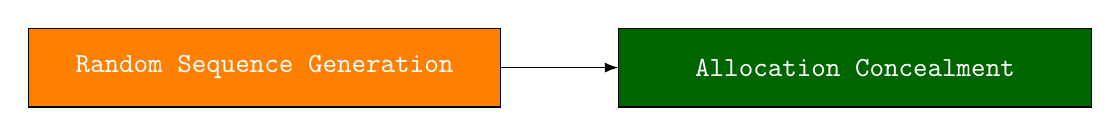
\begin{tikzpicture}[
    node distance=7.5cm,
    box/.style={draw, text=white, minimum width=6cm, minimum height=1cm, font=\ttfamily}
]
    % Nodes
   \node[box, fill=orange] (head) {\textbf{Random Sequence Generation}};
    \node[box, right of=head, fill=darkgreen] (n1) {\textbf{Allocation Concealment}};

    % Arrows
    \draw[-{Latex}] (head) -- (n1);
\end{tikzpicture}
\end{center}


\subsection{SNOSE}

SNOSE stands for \textbf{Sequentially Numbered}, \textbf{Opaque}, \textbf{Sealed} Envelopes - it is a standardized and reliable method of ensuring allocation concealment in clinical trials. 

The components of SNOSE are
\begin{itemize}
\item \textit{Sequentially Numbered} : Each envelope has a unique number, ensuring participants are assigned in a particular order without any skipping.
\item \textit{Opaque} : The envelope is made of thick, non-transparent material, prevents seeing through the envelope to guess the assignment.
\item \textit{Sealed} : The envelope is securely closed to prevent tampering or pre-mature opening.
\end{itemize}

The entire process must be strictly monitored to prevent any tampering and to make the study a reliable one, free of any manipulation. However, SNOSE is not ideal for large trials, computerized randomization systems are preferred there.

\newpage

\section{Blindness}

In any clinical trial, bias is one of the main concerns. Bias may be defined as systematic error, or ``difference between the true value and that actually obtained due to all causes other than sampling variability". It can be caused by conscious factors, subconscious factors, or both. Bias can occur at a number of places in a clinical 
trial, from the initial design through data analysis and interpretation. One general solution to the problem of bias is to keep the participant and the investigator blinded, or masked, to the identity of the assigned intervention.

\subsection{Single-blind}

In a single-blind study, the participants are not aware of which intervention they are receiving. The researcher avoids the problems of biased participant reporting.

\begin{figure}[!htbp]
\centering
\includegraphics[scale=0.3]{single_blind_study}
\end{figure}


\subsection{Double-blind}

In a double-blind study, neither the participants nor the researchers responsible for following the participants, collecting data, and assessing outcomes should know the identity of the intervention assignment. The main advantage of a truly double-blind study is that the risk of bias is reduced.

\begin{figure}[!htbp]
\centering
\includegraphics[scale=0.3]{double_blind_study}
\end{figure}

\subsection{Triple-blind}

A triple-blind study is an extension of the double-blind design where along with the participants and the researchers, the data analysts or the committee monitoring the response variables are not made aware of the intervention assignment. A triple-blind study has the theoretical advantage of allowing the monitoring committee to evaluate the response variable results more objectively. However, in a trial where the monitoring committee has an ethical responsibility to ensure participant safety, such a design may be counter-productive.

\begin{figure}[!htbp]
\centering
\includegraphics[scale=0.3]{triple_blind_study}
\end{figure}

\end{document}